\begin{figure}[t]
    \centering
    \begin{minipage}{1.0\linewidth}
    \small
    \textbf{\hspace{14mm} Topics in \longfact{}.} \\[1ex]
    \begin{adjustbox}{valign=c}
    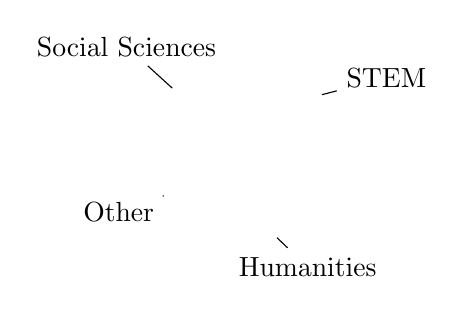
\begin{tikzpicture}[scale=0.4]
        \pie[
            rotate=232,
            sum=auto,
            color={frenchblue!75,frenchrose!75,frenchlilac!75,frenchbeige!75},
        ]{
            11/,
            12/,
            11/,
            4/
        }
        % Add labels
        \node (ss) at (0:0cm) [xshift=-15mm, yshift=13mm] {Social Sciences};
        \node (hum) at (0:0cm) [xshift=8mm, yshift=-15mm] {Humanities};
        \node (stem) at (0:0cm) [xshift=18mm, yshift=9mm] {STEM};
        \node (other) at (0:0cm) [xshift=-16mm, yshift=-8mm] {Other};
        % Draw lines to pie slices
        \draw (ss) -- (140:30mm);
        \draw (hum) -- (290:30mm);
        \draw (stem) -- (35:30mm);
        \draw (other) -- (210:30mm);
    \end{tikzpicture}
    \end{adjustbox}
    \small
    \begin{adjustbox}{valign=c}
    \vspace{-50mm}
    \begin{tabular}{l | cc}
        \toprule
        Factuality Benchmark & \# Topics & Response type \\
        \midrule
        TruthfulQA \citep{lin2022truthfulqa}        & 38        &   Short-answer \\
        HaluEval \citep{li2023halueval}             & Many      &   Short-answer \\
        FreshQA \citep{vu2023freshllms}             & Many      &   Short-answer \\
        HalluQA \citep{cheng2023evaluating}         & 14        &   Short-answer \\
        FELM \citep{chen2023felm}                   & 5         &   Mixed \\
        FActScore \citep{min2023factscore}          & 1         &   Long-form \\
        \textbf{LongFact (ours)}                    & 38        &   Long-form \\
        \bottomrule
    \end{tabular}
    \end{adjustbox}
    \end{minipage}
    \caption{
        We present \longfact{}, a prompt set designed to probe a model's factuality when generating long-form responses.
        Left: \longfact{} consists of 38 topics (listed in \cref{sec:longfact-list-of-topics}) categorized into four supercategories.
        Right: compared to existing factuality datasets, \longfact{} (a) tests long-form responses rather than short answers and (b) covers a broad range of topics.
    }
    \label{fig:longfact-main-figure}
    \vspace{-2mm}
\end{figure}